\documentclass{article}
\usepackage[a4paper]{geometry}
\usepackage[utf8]{inputenc}
\usepackage{polski}
\usepackage{tabularx}
\usepackage{indentfirst}
\usepackage{multirow}
\usepackage{amssymb}
\usepackage{amsmath}
\usepackage{anysize}
\usepackage{float}
\usepackage{caption}
\usepackage{subcaption}
\usepackage{graphicx}

\usepackage{listings}
\usepackage{color}
\lstset{literate=%
{ą}{{\k{a}}}1 {ć}{{\'c}}1 {ę}{{\k{e}}}1 {ł}{{\l{}}}1 {ń}{{\'n}}1 {ó}{{\'o}}1 {ś}{{\'s}}1 {ż}{{\.z}}1 {ź}{{\'z}}1 {Ą}{{\k{A}}}1 {Ć}{{\'C}}1 {Ę}{{\k{E}}}1 {Ł}{{\L{}}}1 {Ń}{{\'N}}1 {Ó}{{\'O}}1 {Ś}{{\'S}}1 {Ż}{{\.Z}}1 {Ź}{{\'Z}}1 }

\definecolor{mygreen}{rgb}{0,0.6,0}
\definecolor{mygray}{rgb}{0.5,0.5,0.5}
\definecolor{mymauve}{rgb}{0.58,0,0.82}

\usepackage{titling}
\newcommand{\subtitle}[1]{%
	\posttitle{%
	\par\end{center}
	\begin{center}\small#1\end{center}
	\vskip0.5em}%
}

\title{Algenic -- serwis z~konkursami algorytmicznymi}
\subtitle{Akademia Górniczo-Hutnicza im. Stanisława Staszica w Krakowie\\
	Wydział Elektrotechniki, Automatyki,\\
	Informatyki i Inżynierii Biomedycznej}
\author{Kacper Tonia\and
		Sławomir Kalandyk\and
		Mateusz Ruciński}
\date{}

\begin{document}
%------------------------------------------------------------
\maketitle
%------------------------------------------------------------
\section{Wstęp}
System z konkursami algorytmicznymi Algenic służy do hostowania konkursów algorytmicznych. Umożliwia zdalną kompilację przysłanych rozwiązań zadań oraz wyświetlanie wyników tej kompilacji.

\section{Architektura}

\begin{figure}[H]
	\centering
	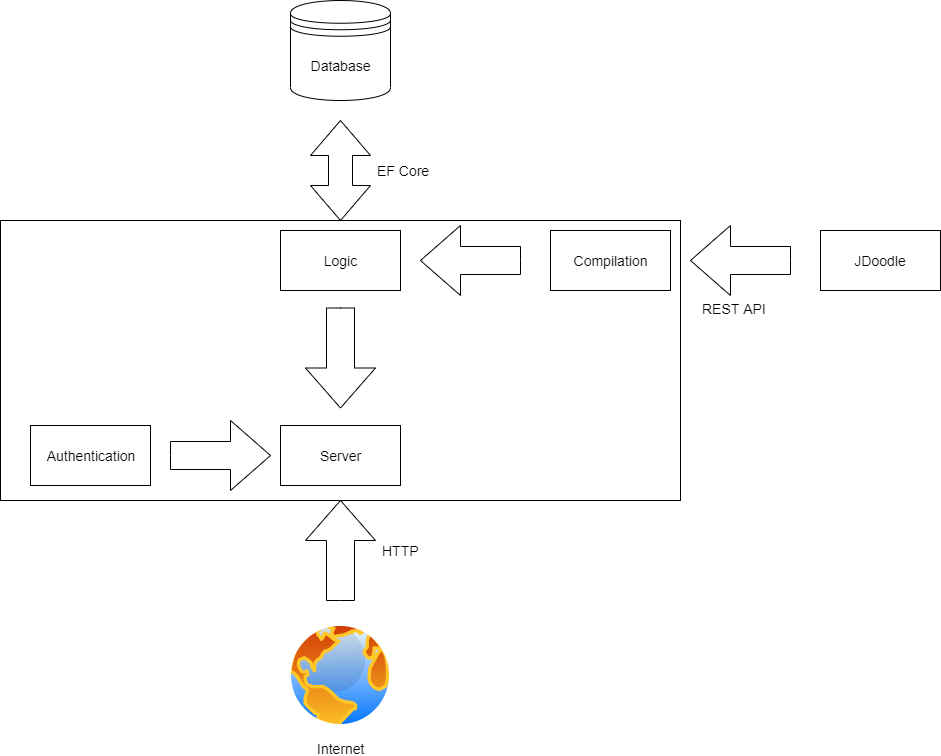
\includegraphics[width=\linewidth]{project_modules.png}
	\caption{Ogólny diagram modułów}
\end{figure}

\section{Baza danych}
\begin{figure}[H]
	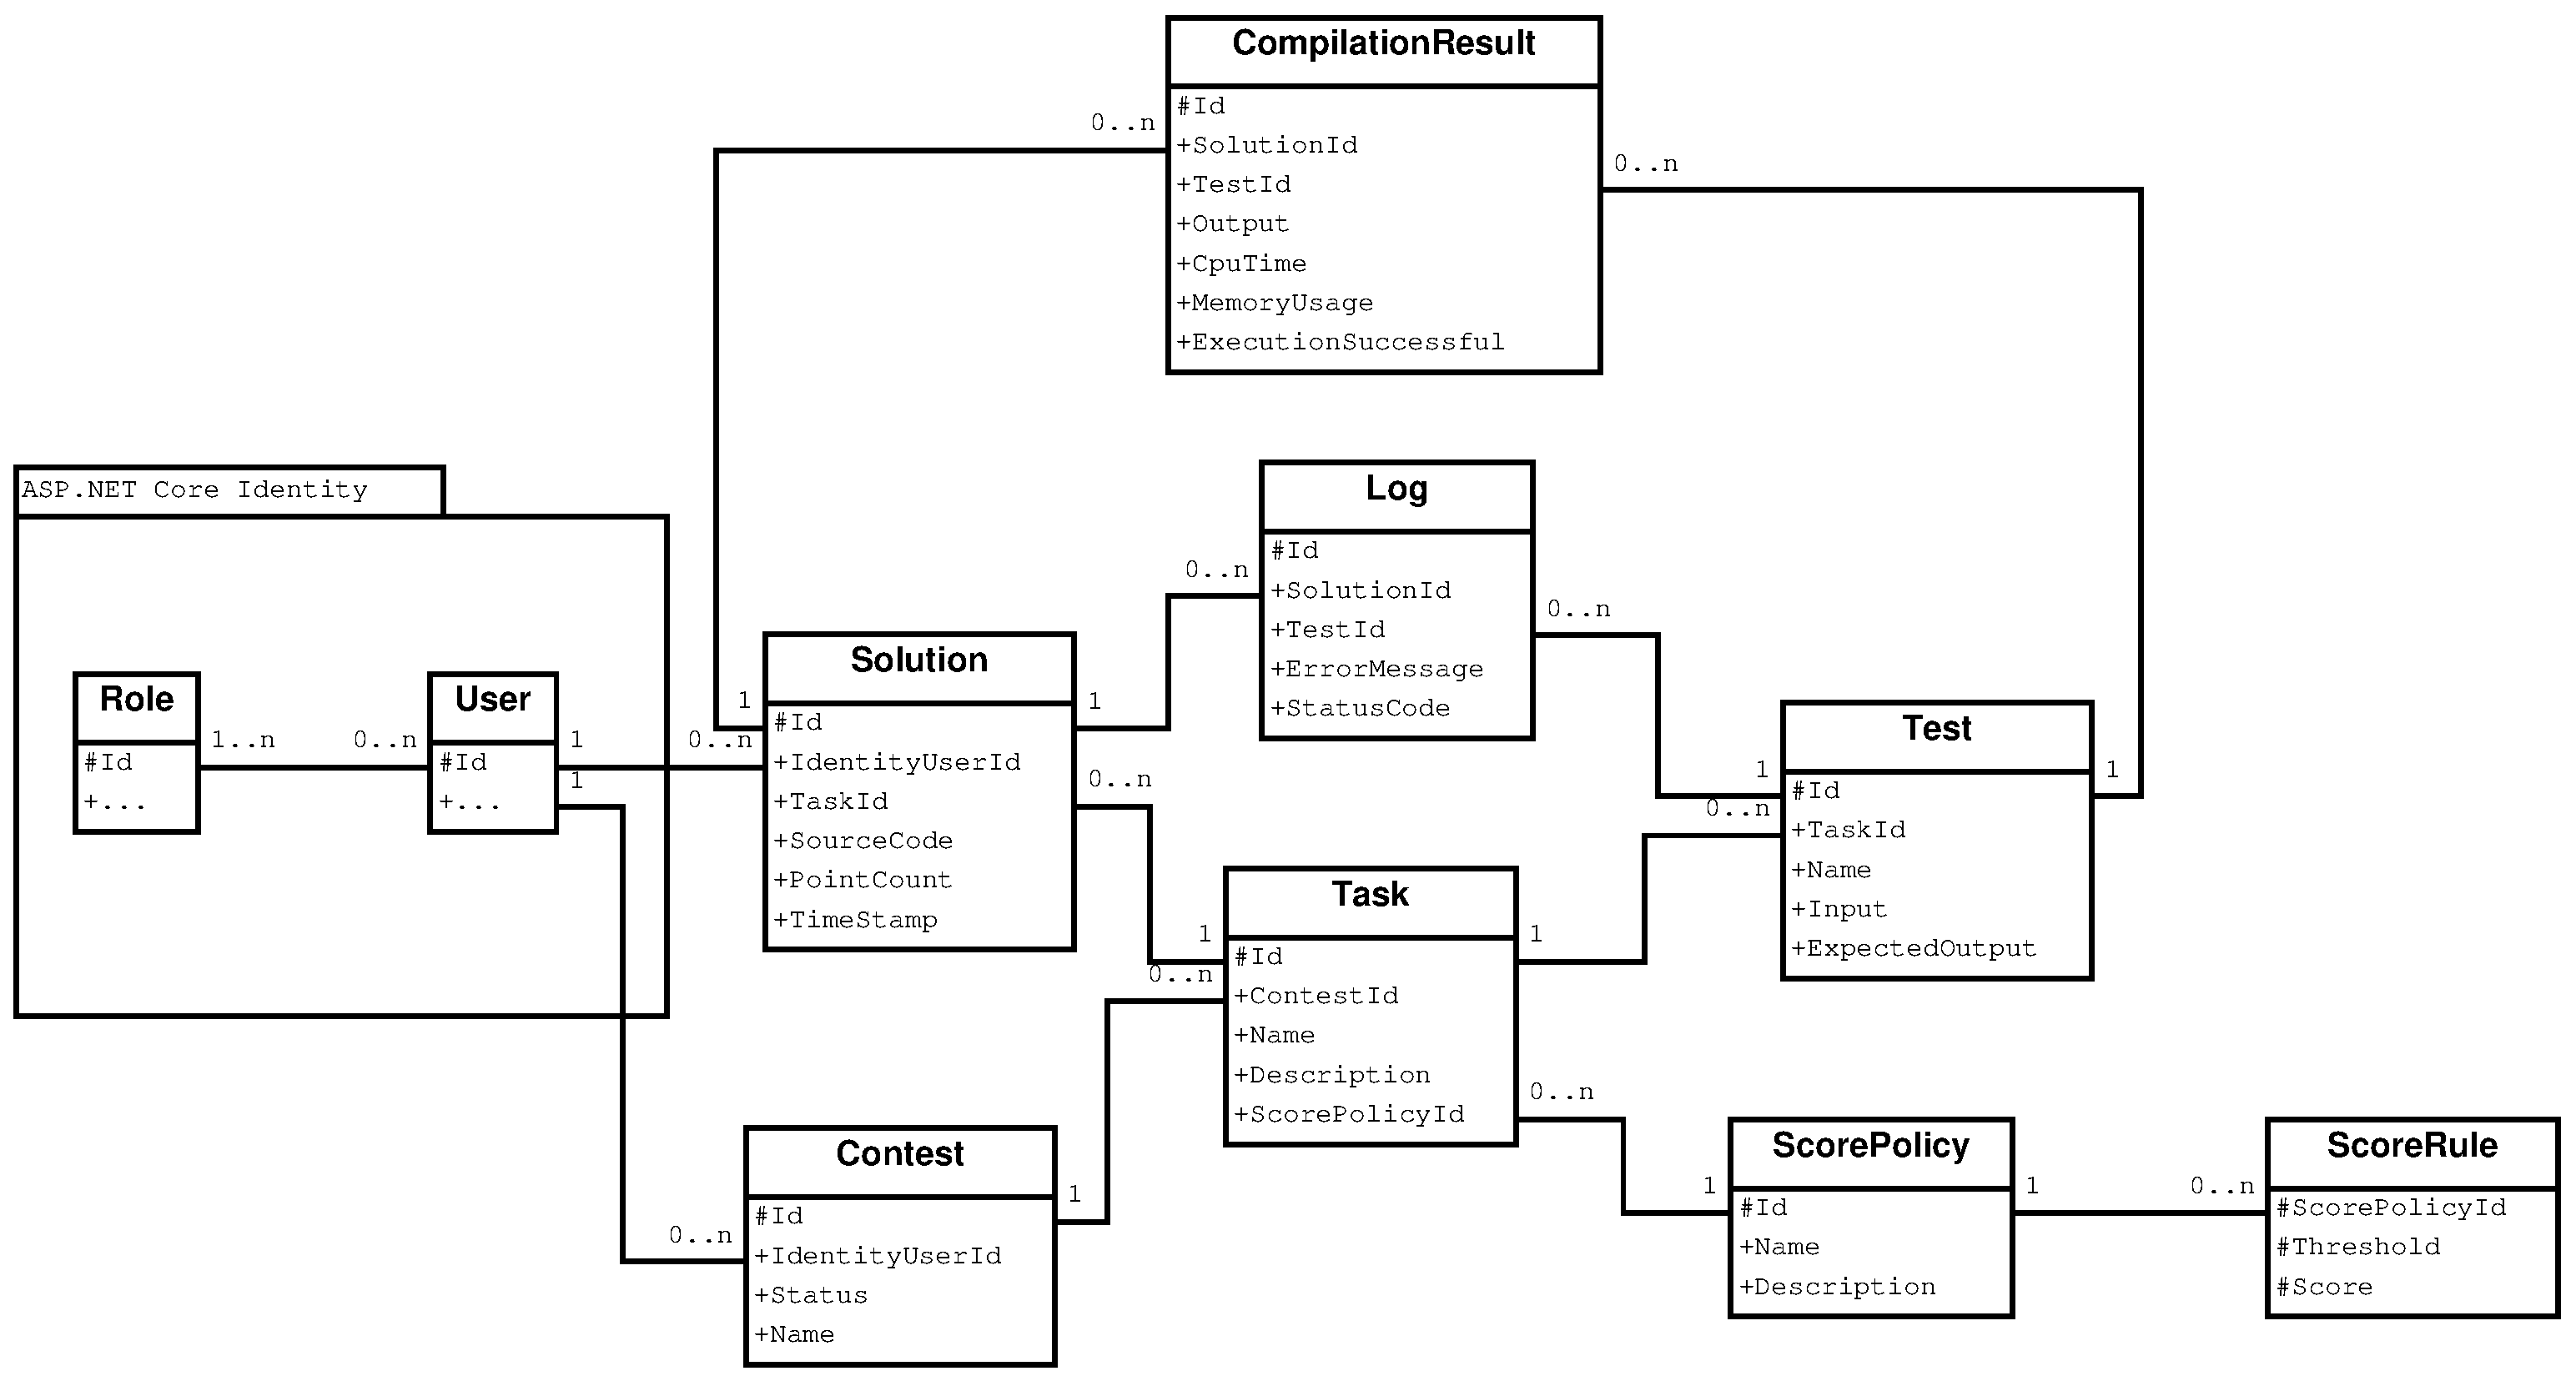
\includegraphics[width=\linewidth]{entityDiagram.eps}
	\caption{Diagram obecnej bazy danych}
\end{figure}

Baza danych jest generowana za pomocą narzędzi dostarczanych przez Entity Framework Core. Przy uprzednim utworzeniu modelu oraz klas konfigurujących własności tabel (n.p. klucze obce), można wygenerować migrację funkcją add-migration i utworzyć lub dokonać zmian w istniejącej bazie danych funkcją update-database. Obie te czynności muszą być wykonane z poziomu konsoli. 

W razie wszelkich błędów przy aktualizacji bazy danych, istnieje możliwość ręcznego modyfikowania migracji.

\section{Role użytkowników}
\subsection{Wspólne}
\begin{itemize}
    \item Każdy użytkownik ma możliwość zarejestrowania się w aplikacji i zalogowania
    \item Każdy użytkownik może zobaczyć aktualnie trwające lub zakończone konkursy
\end{itemize}

\subsection{Podstawowy użytkownik}
\begin{itemize}
    \item Może dołączyć do konkursu
    \item Po dołączeniu do konkursu może wyświetlać znajdujące się w nim zadania i przesyłać rozwiązania do nich
\end{itemize}

\subsection{Egzaminator}
\begin{itemize}
    \item Posiada możliwości podstawowego użytkownika
    \item Może tworzyć konkursy
    \item Po utworzeniu konkursu może dodawać do niego zadania
    \item Po dodaniu zadania może dodawać do niego testy
    \item Ma możliwośc zmiany stanu swoich konkursów (n.p. po dodaniu zadań może go wystartować, a później zakończyć)
    \item Uruchamia kompilację rozwiązań zadań konkursowych po zakończeniu swojego konkursu (WIP)
    \item Dodaje listę par postaci (próg procentowy, ilość punktów), według której ocenianie jest zadanie (WIP)
\end{itemize}

\subsection{Administrator}
\begin{itemize}
    \item Posiada możliwości podstawowego użytkownika oraz egzaminatora
    \item Może modyfikować uprawnienia innych użytkowników (WIP)
\end{itemize}

\section{Technologia i~narzędzia}

\textbf{Język programowania:} C\#

\textbf{Framework:} ASP.NET~Core~2.2

\textbf{System kontroli wersji:} Git

\textbf{Platforma:} GitHub

\textbf{Serwis do testów automatycznych:} Travis CI

\textbf{Framework do testów jednostkowych:} xunit

\textbf{Framework do testów funkcjonalnych:} Selenium WebDriver

\textbf{Zdalna kompilacja:} JDoodle

Projekt został oparty o~framework ASP.NET~Core ze~względu na~jego popularność, wieloplatformowość i~fakt bycia oprogramowiem typu open source. Zrezygnowaliśmy z~sięgnięcia po~najnowszą wersję frameworka,~3.0, na~rzecz bardziej dojrzałej i~potencjalnie stabilniejszej wersji~2.2.

Rozważyliśmy wykorzystanie usługi Azure, co~pozwoliłoby na~skupienie większości aspektów pracy nad~programem w~jednym miejscu (począwszy od~przechowywania plików projektu, poprzez zarządzanie bazą danych projektu, skończywszy na~automatycznym testowaniu zmian i~wdrażaniu aktualnej wersji aplikacji w~chmurze Azure). Stosunkowo długie czasy testowania i~wdrażania w~chmurze, a~także względnie niewielka złożoność naszego projektu sprawiły, że~zdecydowaliśmy się na~uruchamianie~i~testowanie aplikacji lokalnie, wraz z~lokalną bazą danych w~technologii SQL~Server.

Ostatecznie wybraliśmy platformę GitHub m.in.~ze~względu na~wbudowane narzędzia do~zarządzania projektem, takie jak tablica zadań, które ułatwią systematyzację zadań związanym z~etapem implementacji i~przydzielanie owych zadań członkom zespołu. Jako element praktyki \emph{Continuous Integration}, zmiany dodawane do~głównego repozytorium są~automatycznie testowane na~platformie \textbf{Travis~CI}.

Na~późniejszym etapie prac nad projektem możemy ponownie rozważyć wykorzystanie Azure, chociażby w~celu uruchomienia wspólnej, trwałej bazy danych w~chmurze.

W~celu kompilowania kodów przysyłanych przez użytkowników wykorzystamy serwis \textbf{JDoodle}, oferujący REST-owe API do~zdalnej kompilacji. Kompilowanie niezaufanego kodu na~serwerze niosłoby poważne zagrożenie, o~ile nie podjęlibyśmy specjalnych środków bezpieczeństwa. Użycie istniejącej usługi jak JDoodle redukuje potencjalne problemy z~bezpieczeństwem.

W~darmowym wariancie JDoodle pozwala na~przeprowadzenie ok.~200 kompilacji dziennie. Może być to~zbyt mała wartość podczas intensywnego testowania, jednak prostota użycia i~bogata ilość dostępnych języków programowania przekonuje nas ostatecznie do~owego rozwiązania.

%------------------------------------------------------------
\section{Analiza ryzyka}


\begin{figure}[H]
	\centering
	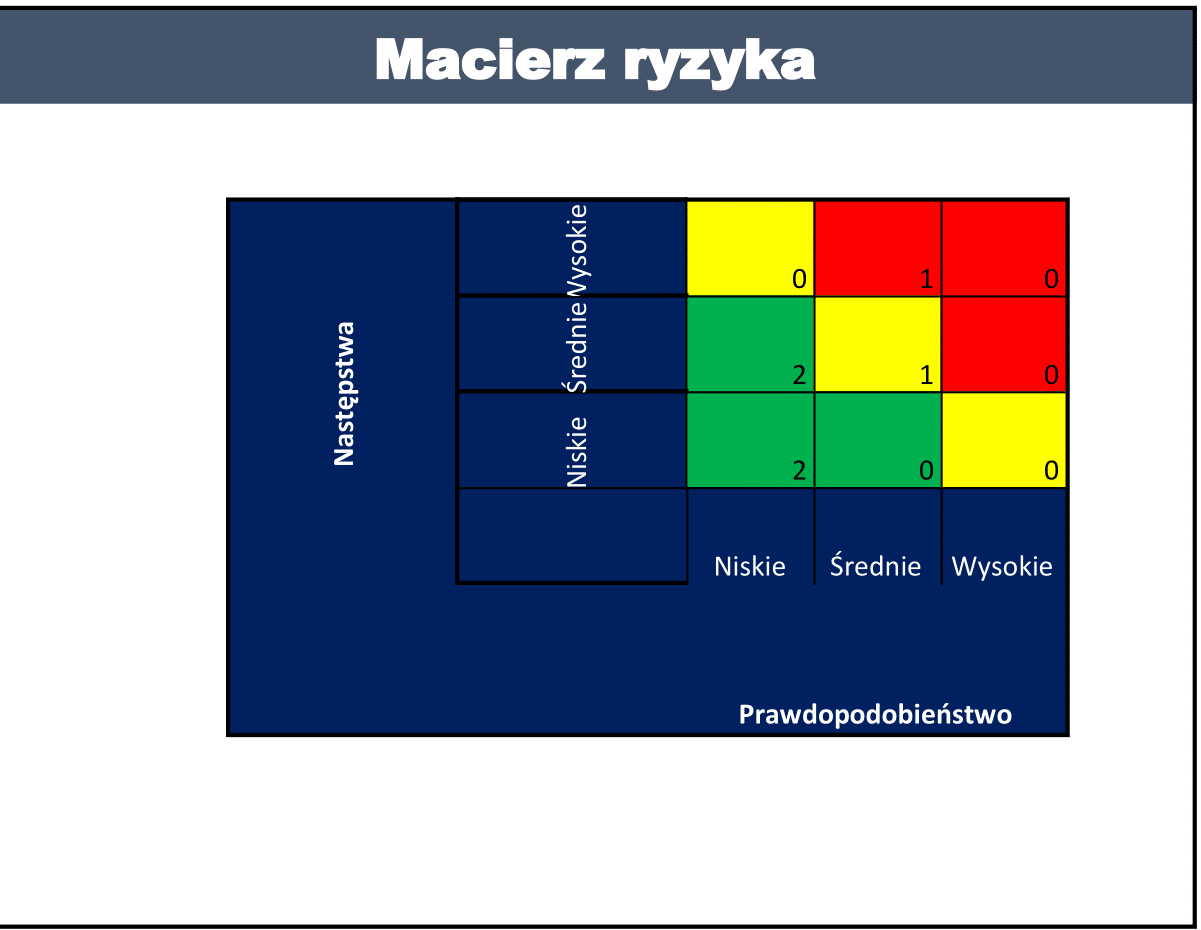
\includegraphics[width=.5\linewidth]{macierz_ryzyka.png}
	\caption{Macierz ryzyka}
\end{figure}

Macierz ryzyka tworzymy w celu określenia poziomu ryzyka związanego z~produkcją i~działaniem produktu w celu obniżenia negatywnego wpływu ryzyka na~funkcjonowanie danego podmiotu i~podejmowanie odpowiednich działań służących przeciwdziałaniu i~ograniczaniu ryzyka. Po~stworzeniu listy ryzyk i~oszacowaniu ryzyka dla każdego elementu z~listy można wywnioskować, że~najwyższe ryzyko jest związane z~błędem ludzkim (programisty). Minimalizować to~ryzyko możemy, testując oprogramowanie przed wdrożeniem oraz dbać o~obecność backupów na~wypadek problemów z~aktualizacją.

\begin{figure}[H]
	\centering
	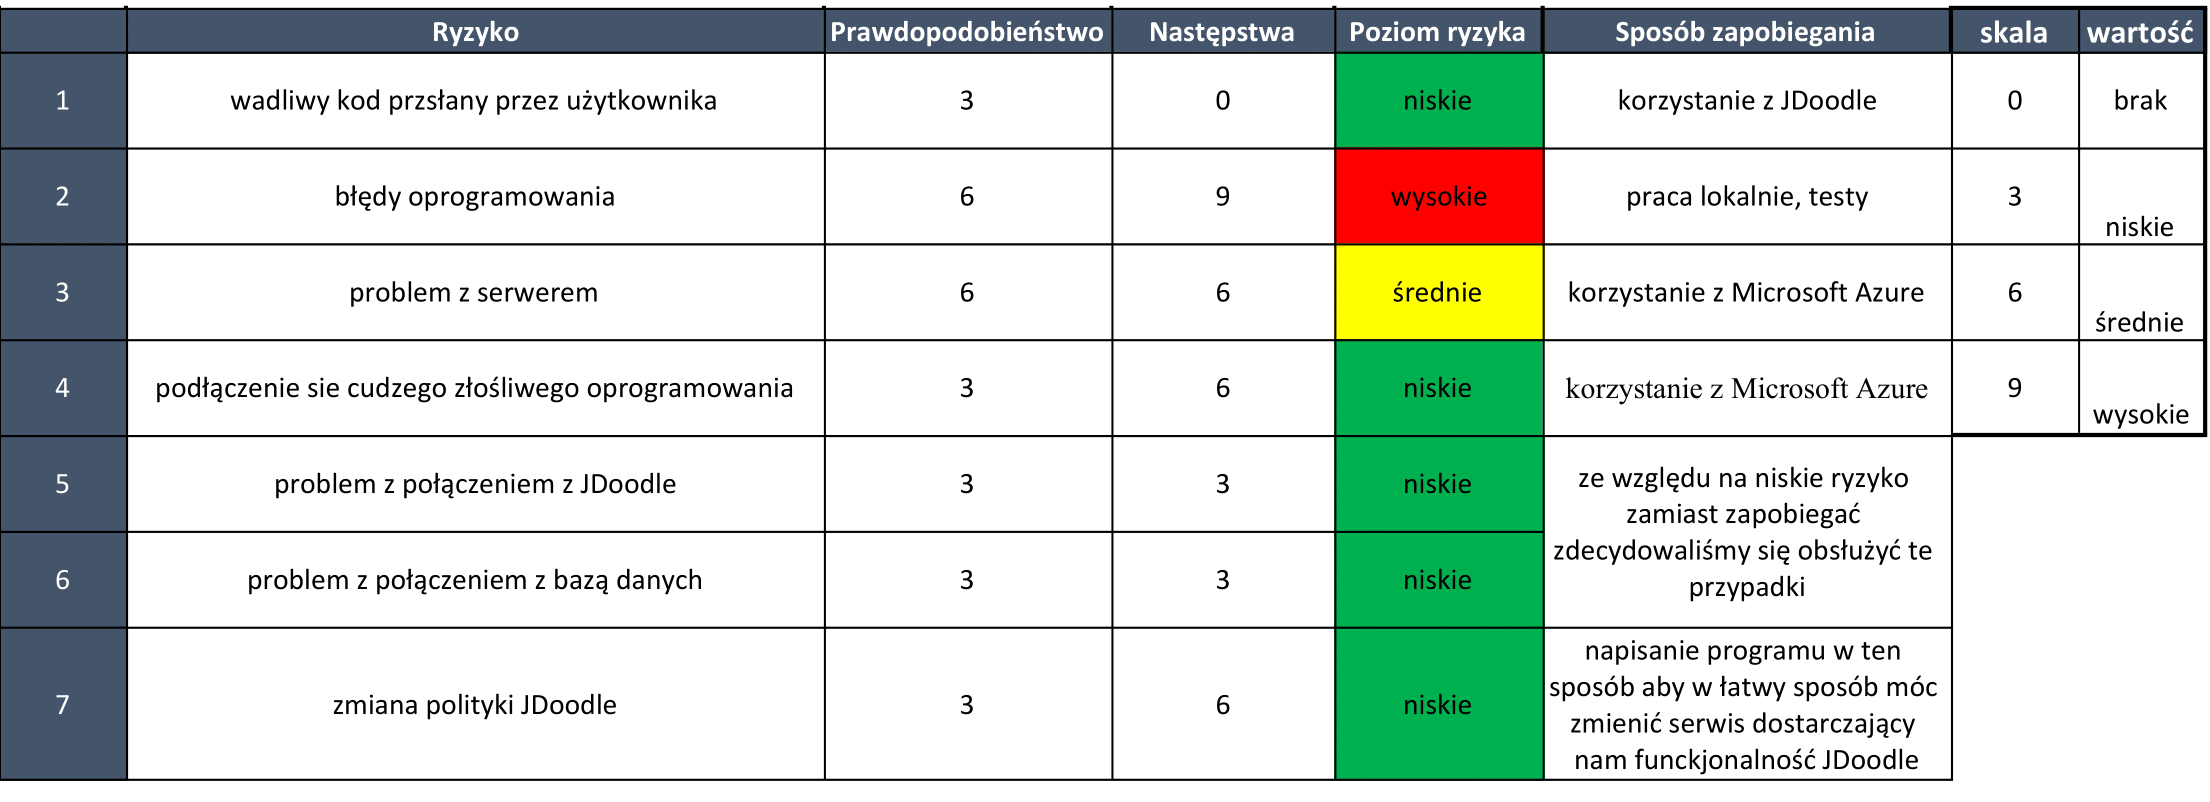
\includegraphics[width=.95\linewidth]{lista_ryzyk.png}
	\caption{Lista ryzyk}
\end{figure}

\section{Implementacja}
\subsection{Stany konkursu}
\begin{itemize}
    \item Nierozpoczęty
    \begin{itemize}
        \item Egzaminator może zmienić stan konkursu na W trakcie
        \item Egzaminator może dodawać i edytować zadania
        \item Użytkownicy mogą obejrzeć konkurs, ale nie mogą przejrzeć zadań
    \end{itemize}

    \item W trakcie
    \begin{itemize}
        \item Egzaminator może zmienić stan konkursu na Nierozpoczęty lub Zakończony
        \item Egzaminator może dodawać i edytować zadania
        \item Użytkownicy mogą rozwiązywać zadania
    \end{itemize}

    \item Zakończony
    \begin{itemize}
        \item Egzaminator może zmienić stan konkursu na W trakcie
        \item Nie można dodawać ani modyfikować zadań
    \end{itemize}
\end{itemize}

\subsection{Wspierane języki programowania}
\begin{itemize}
    \item C++ (GCC 9.1.0)
    \item C (GCC 9.1.0)
    \item Java (JDK 11.0.4)
\end{itemize}

\end{document}